% !TEX program = xelatex
% UMI, RSS 2024 pp. 4-6; project appendix A,D,E,F.
% Hybrid composition. Unmodified built-in imagegen illustration viewports only.
% All text/formulas/external causal arrows below are independent TikZ/TeX.
% Relative-transform equation expands source prose; not an original numbered equation.
% Noise-prediction loss is standard Diffusion Policy teaching, not a new UMI loss.
\documentclass[tikz,border=0bp]{standalone}
\usepackage{lmodern}
\usepackage{fontspec,xeCJK,amsmath,amssymb,graphicx}
\setsansfont{Arial}
\setCJKmainfont[Path=/System/Library/Fonts/,BoldFont={STHeiti Medium.ttc}]{STHeiti Light.ttc}
\setCJKsansfont[Path=/System/Library/Fonts/,BoldFont={STHeiti Medium.ttc}]{STHeiti Light.ttc}
\renewcommand{\familydefault}{\sfdefault}
\usetikzlibrary{arrows.meta,calc}
\definecolor{ink}{HTML}{173646}
\definecolor{teal}{HTML}{167D81}
\definecolor{amber}{HTML}{AD7425}
\definecolor{navy}{HTML}{314976}
\definecolor{pale}{HTML}{F2F8F7}
\definecolor{warm}{HTML}{FFF7E9}
\definecolor{blue}{HTML}{F2F5FB}
\tikzset{txt/.style={text=ink,font=\fontsize{14}{18}\selectfont,align=center,inner sep=0},hd/.style={txt,font=\bfseries\fontsize{17}{21}\selectfont},sm/.style={txt,font=\fontsize{13.5}{17}\selectfont},a/.style={-{Stealth[length=5bp,width=4bp]},line width=1.3bp,draw=teal,rounded corners=3bp},train/.style={a,draw=amber,dashed},box/.style={rounded corners=8bp,line width=.9bp}}
\newcommand{\txt}[4]{\node[txt,text width=#3bp]at(#1,#2){#4};}
\newcommand{\smalltxt}[4]{\node[sm,text width=#3bp]at(#1,#2){#4};}
\newcommand{\head}[4]{\node[hd,text width=#3bp]at(#1,#2){#4};}
\newcommand{\panel}[5]{\draw[box,draw=#4!55,fill=#5](10,#1)rectangle(330,#2);\node[hd,anchor=west,text=#4]at(22,#1+21){#3};}
% Source PNG is 1086x1448 px at 72 dpi natural bbox. Coordinates are pixels.
\newcommand{\art}[7]{\begingroup\pgfmathsetmacro{\bt}{1448-#2-#4}\pgfmathsetmacro{\rt}{1086-#1-#3}\node[anchor=north west,inner sep=0]at(#5,#6){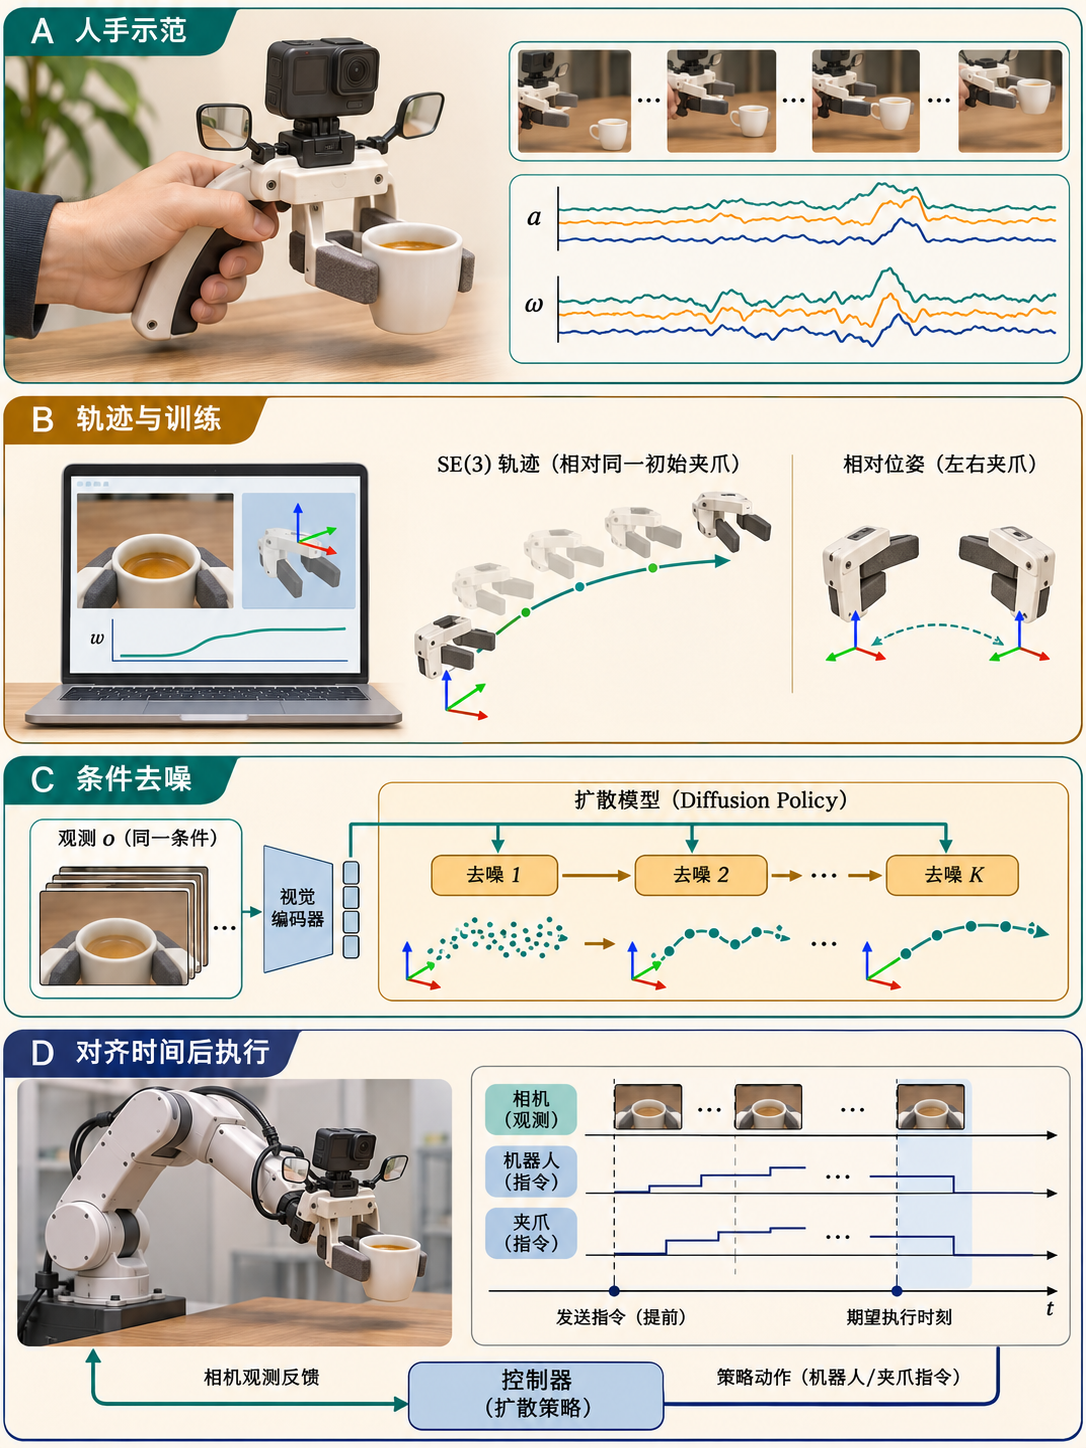
\includegraphics[trim=#1bp \bt bp \rt bp #2bp,clip,width=#7bp]{umi-imagegen-draft.png}};\endgroup}
\begin{document}
\begin{tikzpicture}[x=1bp,y=-1bp]
\path[use as bounding box](0,0)rectangle(340,1230);\fill[white](0,0)rectangle(340,1230);
\head{170}{17}{330}{UMI：人手示范怎样交给机器人？}
\smalltxt{170}{42}{320}{训练：A → B → C\qquad 部署：C → D 闭环}
\panel{65}{254}{A\quad 人手采集}{teal}{pale}
% Polygon removes the old top-left title while preserving complete camera top.
\begin{scope}\clip(91,104)--(170,104)--(170,212.3)--(18,212.3)--(18,112)--(91,112)--cycle;\art{8}{34}{480}{342}{18}{104}{152}\end{scope}
\txt{250}{131}{140}{GoPro 鱼眼 RGB\\+ 内置 IMU}
\txt{250}{183}{140}{侧镜保留视差\\手指控制开合}
\txt{170}{233}{295}{RGB + IMU → 录成 MP4}
\draw[train](170,254)--(170,274);
\panel{276}{568}{B\quad 离线恢复动作标签}{amber}{warm}
\txt{170}{325}{300}{视觉惯性 SLAM → 米制位姿}
\txt{170}{350}{300}{指间标记 → 连续夹爪宽度}
\art{414}{487}{359}{231}{24}{369}{164}
\art{819}{520}{240}{150}{204}{390}{110}
\smalltxt{107}{487}{170}{共用当前起点 $T_0$}
\smalltxt{260}{478}{120}{双臂相对位姿}
\node[txt]at(170,516){$\displaystyle \Delta T_{0\to t}=T_0^{-1}T_t$};
\smalltxt{170}{547}{302}{机器人运动学 → 过滤不可行轨迹}
\draw[train](170,568)--(170,588);
\panel{590}{916}{C\quad 条件 Diffusion Policy}{teal}{pale}
\txt{170}{640}{302}{条件 $c$：图像、相对位姿、宽度历史}
\smalltxt{170}{664}{300}{双臂任务另加入两夹爪相对位姿}
\draw[box,draw=amber!50,fill=warm](22,684)rectangle(318,787);
\smalltxt{170}{701}{280}{训练：动作加噪得到 $A^{(k)}$}
\node[txt]at(170,729){$\displaystyle \mathcal L=\|\epsilon-\epsilon_\theta(A^{(k)},k,c)\|^2$};
\smalltxt{170}{752}{280}{$k$：扩散步；$\epsilon$：所加噪声}
\smalltxt{170}{774}{280}{噪声预测教学式；误差更新策略 $\theta$}
\txt{170}{811}{292}{推理：随机噪声 + 当前条件 $c$}
\art{397}{908}{658}{82}{27}{829}{286}
\txt{170}{888}{298}{逐轮去噪 → 相对位姿 + 宽度序列}
\draw[a](170,916)--(170,936);
\panel{938}{1218}{D\quad 对齐时钟，闭环执行}{navy}{blue}
\art{18}{1080}{434}{265}{24}{978}{134}
\smalltxt{243}{1012}{143}{测量各路时延\\按目标到达时刻\\调度臂与夹爪}
\txt{170}{1082}{277}{腕部 RGB + 机器人本体反馈}
\draw[a](170,1094)--(170,1105);
\txt{170}{1118}{278}{对齐历史 → C 中策略推理}
\draw[a](170,1130)--(170,1141);
\txt{170}{1154}{278}{丢弃过期目标 → 分别提前发指令}
\draw[a](170,1166)--(170,1177);
\txt{170}{1190}{264}{机械臂 / 夹爪 → 环境}
% Correct runtime feedback is environment -> new observations, not controller -> camera.
\draw[a](283,1190)--(320,1190)--(320,1082)--(309,1082);
\end{tikzpicture}
\end{document}
